\documentclass[a4paper]{article}
\usepackage[utf8]{inputenc}
\usepackage[T1]{fontenc}
\usepackage[french]{babel}
\usepackage{amsmath,amsfonts,amssymb}
\usepackage{bookman}
\usepackage{xcolor}
\usepackage{array}
\usepackage{pifont}
\usepackage{ulem}
\usepackage{listings}
\usepackage{graphicx}
\usepackage{eurosym}
\usepackage[left=2cm, right=2cm, top=2cm, bottom=2cm]{geometry}
\frenchbsetup{StandardLists=true}
\newcommand\coord[3]{\begin{pmatrix}
#1 \\
#2 \\
#3
\end{pmatrix}}
\newcommand{\R}{\mathbb{R}}
\newcommand{\N}{\mathbb{N}}
\newcommand{\D}{\mathbb{D}}
\newcommand{\Z}{\mathbb{Z}}
\newcommand{\Q}{\mathbb{Q}}
\newcommand{\C}{\mathbb{C}}
\newcommand{\K}{\mathbb{K}}
\newcommand{\lra}{\Longrightarrow}
\newcommand{\lla}{\Longleftarrow}
\newcommand{\llra}{\Longleftrightarrow}
\setlength{\textheight}{23.5cm}
\newcommand{\ra}{\rightarrow}
\newcommand{\la}{\leftarrow}

\let\oldsection\section
\renewcommand{\section}[1]{\textcolor{purple}{\oldsection{#1}}}
\let\oldsubsection\subsection
\renewcommand{\subsection}[1]{\textcolor{cyan}{\oldsubsection{#1}}}
\let\oldsubsubsection\subsubsection
\renewcommand{\subsubsection}[1]{\textcolor{green}{\oldsubsubsection{#1}}}
\let\oldtextbf\textbf
\renewcommand{\textbf}[1]{\textcolor{cyan}{\oldtextbf{#1}}}
\let\oldunderline\underline
\renewcommand{\underline}[1]{\textcolor{purple}{\oldunderline{#1}}}
\let\oldtextit\textit
\renewcommand{\textit}[1]{\textcolor{violet}{\oldtextit{#1}}}

\lstset{
    inputencoding=utf8,
    extendedchars=true,
    literate=%
    {é}{{\'{e}}}1
    {è}{{\`{e}}}1
    {ê}{{\^{e}}}1
    {ë}{{\¨{e}}}1
    {û}{{\^{u}}}1
    {ù}{{\`{u}}}1
    {â}{{\^{a}}}1
    {à}{{\`{a}}}1
    {î}{{\^{i}}}1
    {ô}{{\^{o}}}1
    {ç}{{\c{c}}}1
    {Ç}{{\c{C}}}1
    {É}{{\'{E}}}1
    {Ê}{{\^{E}}}1
    {À}{{\`{A}}}1
    {Â}{{\^{A}}}1
    {Î}{{\^{I}}}1,
    basicstyle=\footnotesize\sffamily\color{black},
    commentstyle=\textcolor{gray},
    numbers=left,
    numbersep=5pt,
    numberstyle=\textcolor{gray},
    keywordstyle=\textcolor{teal},
    showspaces=false,
    showstringspaces=false,
    stringstyle=\textcolor{magenta},
    tabsize=2
}

\title{Time Bomb: Deuxième rapport}
\author{Ilias Deligiannis, Florent Weber, Nadjib Belaribi, Danyl El-Kabir,\\
Leonardo Nassabain, François Grabenstaetter}

\begin{document}
\sffamily
\everymath{\displaystyle}
\setlength\parindent{0mm}
\setlength{\parskip}{0.2cm}
\maketitle

\section{État du projet}

Dans l'état actuel du projet, nous avons un noyau entièrement fonctionnel ainsi qu'une interface de test en console qui nous permet de facilement vérifier que le jeu fonctionne correctement, et qui est la même interface que celle utilisée par l'interface graphique. L'architecture du noyau ressemble à ceci:

\begin{center}
    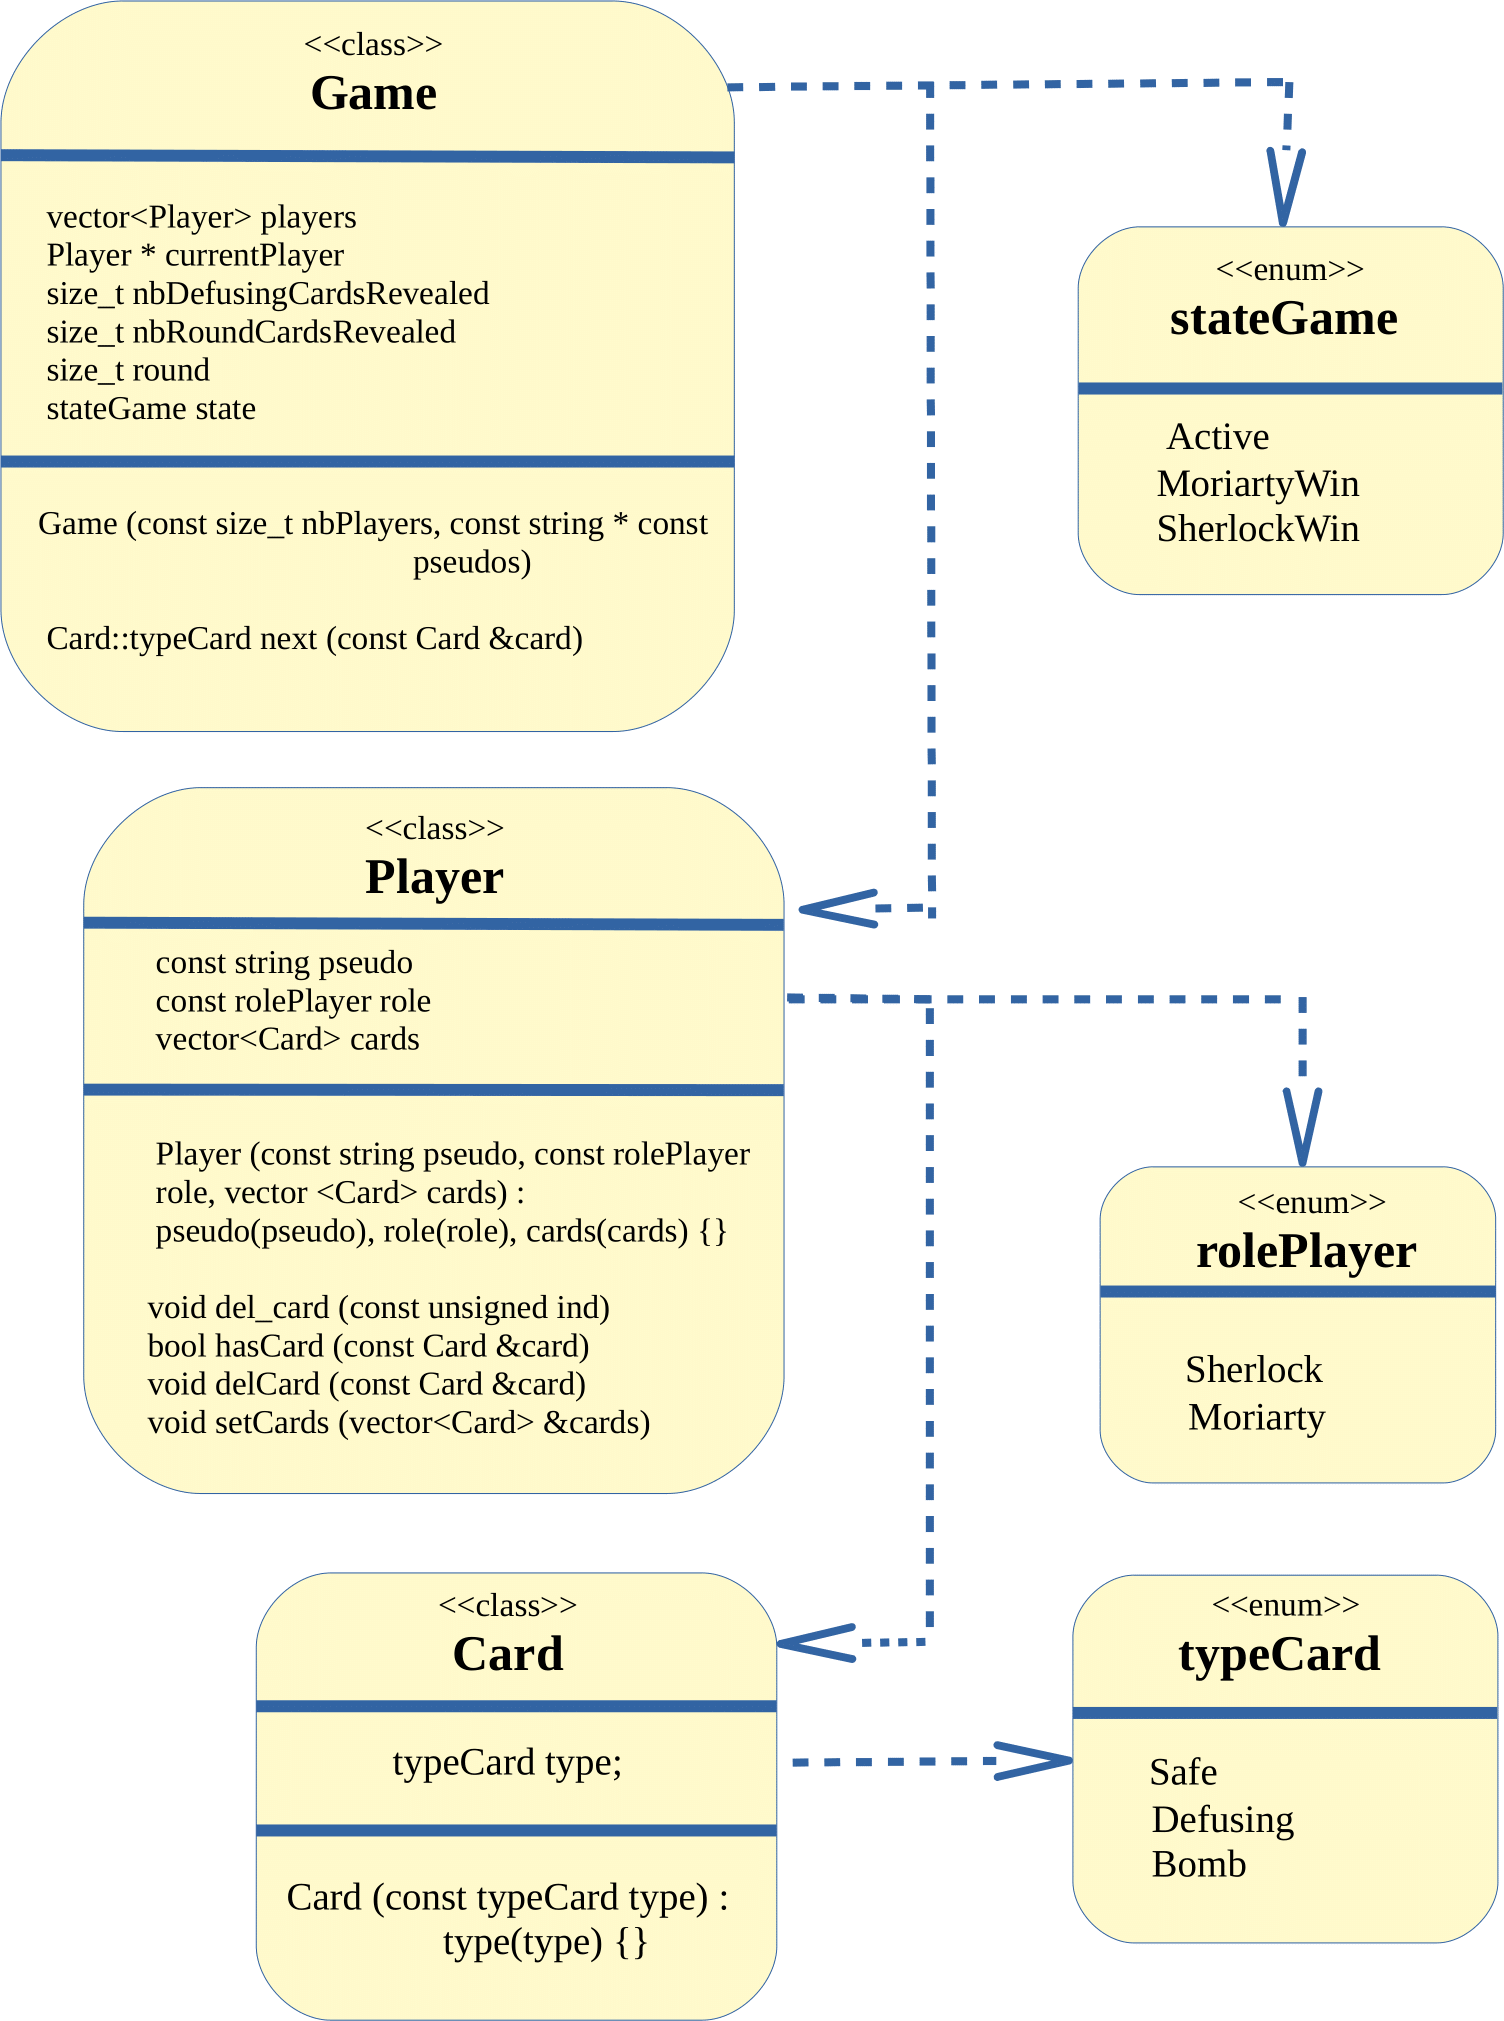
\includegraphics[scale=0.75]{img/diagramme.png}
\end{center}


\section{Interaction avec le noyau depuis l'extérieur}

Chaque module (Interface graphique, Réseau, IA, extensions) pourra communiquer (si implémentés) avec le noyau depuis la classe \textit{Game} (ou par l'intermédiaire d'une classe du module réseau dans le cas d'une partie multijoueurs sur différentes machines).

Nous pouvons distinguer 2 types d'interactions avec le noyau de jeu d'un point de vue du joueur:
\begin{itemize}
    \item Directement avec les méthodes de la classe \textit{Game}. Cette interaction est destinée au jeu en local sur une seule machine pour tous les joueurs, ou bien pour l'hôte (uniquement) lors d'une partie multijoueurs en ligne avec un hôte et des clients qui s'y connectent.
    \item Par l'intermédiaire de la classe \textit{GSocket}, qui représente le module réseau de notre programme. Cette classe permet l'interaction des clients avec l'hôte lors d'une partie multijoueur en ligne. En effet, une seule instance de la classe \textit{Game} est nécessaire pour que le jeu puisse se dérouler.
\end{itemize}

\subsection{L'interaction avec la classe Game}

Le principe de déroulement du jeu est simple:
\begin{enumerate}
    \item Instancier un objet de classe \textit{Game} avec en paramètre le \textit{nombre de joueurs} et un tableau de taille \textit{nombre de joueurs} avec leurs pseudo.
    \item Dans une boucle, appeler la méthode \textit{next} de la classe \textit{Game} avec en paramètre la carte à dévoiler que le joueur du tour actuel (obtenu avec un appel au getter \textit{getCurrentPlayer}) a choisi.
    \item Si le status du jeu est différent de \textit{Active}, cela signifie que soit l'équipe de Moriarty soit celle de Sherlock a gagnée. Il suffit alors de tester cette valeur en fin de boucle avec la méthode \textit{getState}
\end{enumerate}

Tout ce qui est lié à l'affichage de l'état de jeu, au joueur actuel, au nombre de cartes "Defusing" trouvées, au choix de la carte, n'est pas le problème du noyau et doit se faire en fonction de l'état du jeu et des informations accessibles.

\subsection{L'interaction avec le réseau (GSocket)}

Le module réseau n'étant pas encore entièrement en place, nous ne pouvons pas confirmer les détails d'interaction avec la classe \textit{GSocket}. Néanmoins, nous pensons que les points suivants constitueraient un bon fonctionnement:
\begin{enumerate}
    \item Les clients, n'ayant pas instancié d'objet de classe \textit{Game}, doivent communiquer avec l'hôte qui héberge la partie \textit{uniquement} via la classe \textit{GSocket}.
    \item \textit{GSocket} envoie à chaque client les changements dans l'état du jeu tel que le joueur actuel et la dernière carte dévoilée, le status de jeu, ...
    \newpage
    \item Afin d'obtenir plus de détails sur le jeu (nombre de cartes "Defusing" trouvées, numéro de la manche (round), nombre de cartes restantes par joueur, la classe \textit{GSocket} peut implémenter un petit système qui permettra de simuler les variables de jeu et de les modifier selon les changements d'état reçus depuis le réseau (par l'hôte). Cela permettra aux autres modules (partie graphique) de ne pas avoir à s'en préoccuper, et également de ne pas devoir envoyer toutes les données nécessaires par le réseau.
\end{enumerate}

\section{Exemple de programme de test du jeu}

Le programme que nous avons mis au point afin de vérifier que le comportement du noyau est correct, ainsi que de pouvoir jouer à une version très basique du jeu (pas d'affichage des cartes au début du tour, ni du rôle, ...) possède l'interface suivante:

\begin{center}
    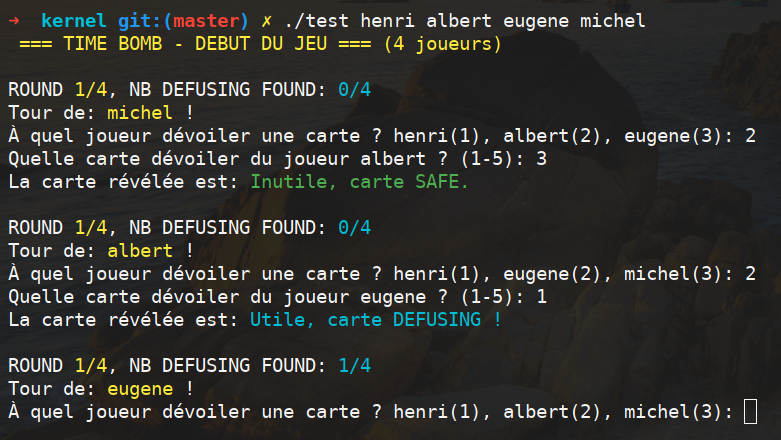
\includegraphics[scale=1.47]{img/test.png}
\end{center}

\begin{center}
    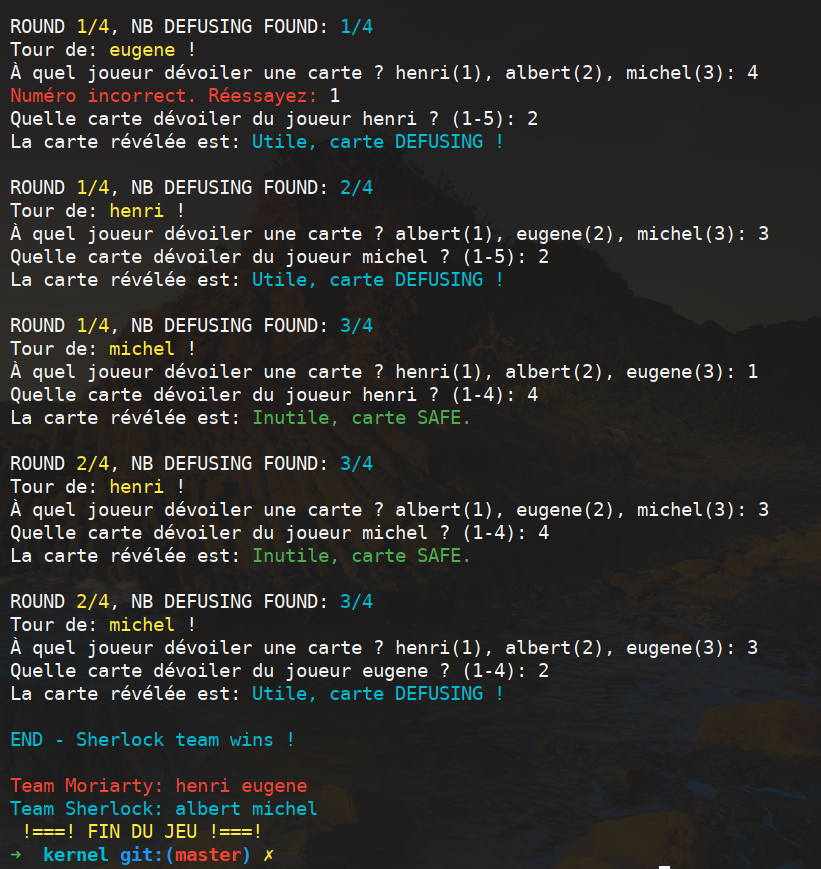
\includegraphics[scale=1.4]{img/fin.png}
\end{center}

\end{document}
